\scanpage{123}
4) \mbox{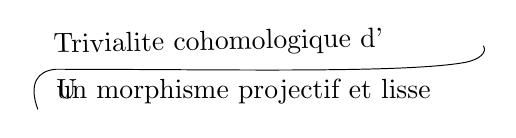
\begin{tikzpicture}[x=1em,y=1em,baseline=(b.base)]
\node[anchor=base west,inner sep=0] (b) at (0,0) {\uline{\rlap{\deleted{U}}\handwritten{u}n morphisme projectif et lisse}};
\node[anchor=base west,inner sep=0,rotate=1] at (-.1,1.65) {\inserted{\handwritten{\uline{Trivialite cohomologique d'}}}};
\draw[line width=.35pt] (-.65,-.4) .. controls (-1.0,.55) and (-.65,1.0) .. (.0,1.05) .. controls (6,1.05) and (12.6,.9) .. (14.8,1.3) .. controls (15.3,1.4) and (15.6,1.65) .. (15.45,1.9);
\end{tikzpicture}} $f:X\handwritten{\longrightarrow}Y$ \uline{de schémas} (correspondant intuitivement à une fibration sur $Y$ à fibres de variétés projectives non singulières). \deleted{est toujours cohomol\unsure{o}giquement} \mbox{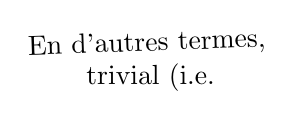
\begin{tikzpicture}[x=1em,y=1em,baseline=(b.base)]
\node[anchor=base west,inner sep=0] (b) at (0,0) {\deleted{trivial (i.e.}};
\node[anchor=base west,inner sep=0,rotate=2] at (-2.1,1.05) {\inserted{\handwritten{En d'autres termes,}}};
\end{tikzpicture}} \rlap{\deleted{l}}\handwritten{L}a suite spectrale de Leray pour la cohomologie $\handwritten{\unsure{\ell|l}}$-adique - ou à coéffi\deleted{\unsure{s}}cients réels dans le cas du corps de base $C$\deleted{)} - \mbox{\resizebox{\linewidth}{!}{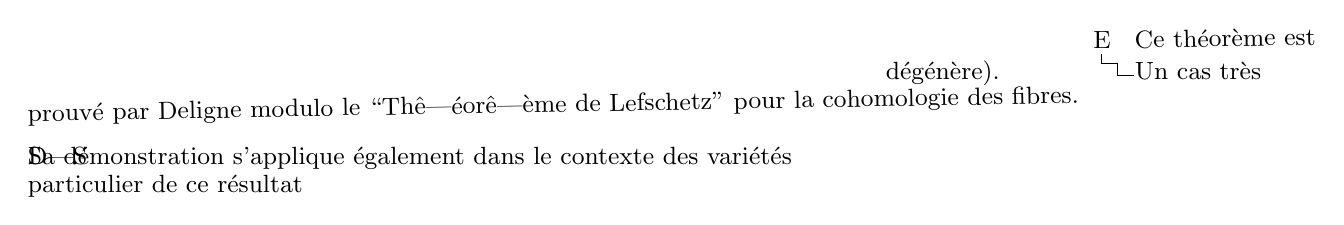
\begin{tikzpicture}[x=1em,y=1em,font=\small]
\node[anchor=base west,inner sep=0] at (31,0) {dégénère\deleted{)}.};
\node[anchor=base west,inner sep=0] at (40,0) {\deleted{Un cas très}};
\node[anchor=base west,inner sep=0] at (38.5,1.15) {\handwritten{\deleted{\unsure{E}}}};
\draw[line width=.45pt] (38.8,.95) -- (38.8,.6) -- (39.4,.6) -- (39.4,.15) -- (40,.15);
\node[anchor=base west,inner sep=0,rotate=1] at (40,1.15) {\inserted{\handwritten{Ce théorème est}}};
\node[anchor=base west,inner sep=0,rotate=1] at (0,-1.5) {\inserted{\handwritten{prouvé par Deligne modulo le ``Th\unsure{ê|é}or\unsure{ê|è}me de Lefschetz'' pour la cohomologie des fibres.}}};
\node[anchor=base west,inner sep=0] at (0,-3.05) {\rlap{\deleted{\unsure{D|S}}}\handwritten{S}a démonstration s'applique également dans le contexte des variétés};
\node[anchor=base west,inner sep=0] at (0,-4.05) {\deleted{particulier de ce résultat}};
\end{tikzpicture}}} analytiques, pour une fibration analytique complexe à fibres compactes kählériennes. Un cas très particulier de ce théorème, relatif au cas où le système local de la cohomologie des fibres était trivial, constitu\mbox{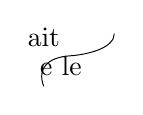
\begin{tikzpicture}[x=1em,y=1em,baseline=(b.base)]
\node[anchor=base west,inner sep=0] (b) at (0,0) {\deleted{e} le};
\node[anchor=base west,inner sep=0] at (-.45,1.05) {\inserted{ait}};
\draw[line width=.35pt] (.15,-.4) .. controls (-.1,.25) and (.3,.65) .. (1.1,.7) .. controls (1.8,.75) and (2.7,1) .. (2.7,1.5);
\end{tikzpicture}} résultat principal de la thèse de Blanchard; mais l'hypothèse de Blanchard n'est réalisée dans presque aucun cas intéressant en géométrie. La démonstration de Deligne est différente bien entendu de celle de Blanchard, que Deligne ne connaissait pas.

Déjà du point de vue transcendant, l'intérêt du résultat de Deligne \deleted{en top} pour la topologie des variétés analytiques est évident. Dans l'optique du rédacteur cependant, ce sont ses implications en géométrie algébrique abstraite,et à longue échéance, à la théorie des nombres, qui sont les plus intéressantes\handwritten{,} \deleted{Par exemple, l\unsure{a|e}} \deleted{et} \rlap{\deleted{\unsure{c}}}\handwritten{C}e sont d'ailleurs des considérations arithmét\unsure{\rlap{q}i|\rlap{i}q}\unsure{\rlap{i}q|\rlap{q}i}ues qui avaient amené le \mbox{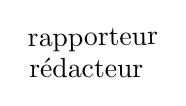
\begin{tikzpicture}[x=1em,y=1em,baseline=(b.base)]
\node[anchor=base west,inner sep=0] (b) at (0,0) {\deleted{rédacteur}};
\node[anchor=base west,inner sep=0,rotate=1] at (-.05,1.1) {\inserted{\handwritten{rapporteur}}};
\end{tikzpicture}} à communiquer à Deligne \deleted{la conjecture} l'énoncé précédent \unsure{\rlap{s}c|\rlap{c}s}omme une conjecture. Grâce au théorème de Deligne, on peut voir par exemple que les hypothèses de R\rlap{\deleted{e}}\handwritten{i}\rlap{\deleted{i}}\handwritten{e}mann-Weil en géométrie diophantienne, interprétées en termes des propriétés d'un endomorphisme de frobénius sur la cohomologie $\handwritten{\unsure{\ell|l}}$-adique, \deleted{restent valables sous une} impliquent des propriétés analogues dans le cas de coéfficients tord\unsure{\rlap{d}u|\rlap{u}d}s (pouvant avoir des singularités quelconques, de plus). Le théorème de Deligne sera un des \mbox{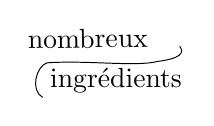
\begin{tikzpicture}[x=1em,y=1em,baseline=(b.base)]
\node[anchor=base west,inner sep=0] (b) at (0,0) {ingrédients};
\node[anchor=base west,inner sep=0,rotate=1] at (-.8,1.4) {\inserted{\handwritten{nombreux}}};
\draw[line width=.35pt] (-.25,-.35) .. controls (-.7,-.1) and (-.5,.75) .. (-.1,.9) .. controls (1.4,1.0) and (3.1,.75) .. (3.9,.95) .. controls (4.7,1.05) and (4.9,1.25) .. (4.7,1.5);
\end{tikzpicture}} techniques \mbox{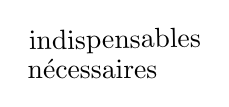
\begin{tikzpicture}[x=1em,y=1em,baseline=(b.base)]
\node[anchor=base west,inner sep=0] (b) at (0,0) {\deleted{nécessaires}};
\node[anchor=base west,inner sep=0,rotate=1] at (.05,1.05) {\inserted{\handwritten{indispensables}}};
\end{tikzpicture}} pour développer la ``théorie des motifs'', qui \handwritten{s}e\rlap{\deleted{\unsure{s}}}\handwritten{\unsure{r}}\rlap{\deleted{\unsure{t}}}\handwritten{a}
% archive sheet number: 122
